\documentclass{beamer}

\title{OAuth: What is it ?}

\usetheme{CambridgeUS}
\usecolortheme{beaver}

\setlength{\itemsep}{10pt}

\begin{document}
	
	\maketitle

	\begin{frame}
		\frametitle{Federated Identity for Single Sign On (SSO)}
		\begin{itemize}
			\setlength{\itemsep}{10pt}
			\item What is Federated Identiry and SSO ?
			\item In this scenario, an end user talks to their Identity Provider (Google, Okta etc.,) and proves ones identity (Authentication)
			\item Identity Provider then generates a cryptographically signed token and hands it off to the application to authenticate the user.
			\item The above federation is based on the trust relationship between Identity Providers and third party services.
			\item OAuth is one of the ways to implement \textbf{Federated Identity}. Another way is \textbf{Security Assertion Markup Language and Protocol (SAML)}
		\end{itemize}
	\end{frame}

	\begin{frame}
		\frametitle{Secure Delegated Access}
		\begin{itemize}
			\setlength{\itemsep}{20pt}
			\item Motivating Example: Yelp wants to know the list of your gmail contacts and check if any of them too are on Yelp
			\item Prior to OAuth and similar standards, users used to provide login and password for their gmail account to Yelp-like services and let them (services) access the account for information.
			\item Clearly, such a sharing of login and password is a risky proposition and a no-no. Need another way of allowing access in a controlled way for a short duration.
		\end{itemize}
	\end{frame}

	\begin{frame}
		\frametitle{Secure Delegated Access...contd}
		\begin{itemize}
			\setlength{\itemsep}{20pt}
			\item For instance, users can allow Yelp to just know the list of contacts and not allow it access to other details.
			\item Besides, access should be limited to a short duration after which the access would stand revoked.
			\item Enter OAuth and similar frameworks/standards. OAuth lets users to allow third party apps to access the user's accounts or data in a controlled fashion. This is called \textbf{Secure Delegated Access/Authorization}
		\end{itemize}
	\end{frame}

	\begin{frame}
		\frametitle{Limitations of SAML for Secure Deleted Authorization}
		From the article 'What the heck is OAuth' by Matt Raible
		\begin{itemize}
			\setlength{\itemsep}{5pt}
			\item SAML is basically a session cookie in your browser that gives you access to webapps. It’s limited in the kinds of device profiles and scenarios you might want to do outside of a web browser.
			\item A lot has changed since SAML was introduced in 2005
			\item Now we have modern web and native application development platforms. There are Single Page Applications (SPAs) like Gmail/Google Inbox, Facebook, and Twitter.
			\item They have different behaviors than your traditional web application, because they make AJAX (background HTTP calls) to APIs.
			\item SAML SSO isn’t particularly good at any of this.
		\end{itemize}
	\end{frame}

	\begin{frame}
		\frametitle{OAuth Central Components}
		OAuth is built on the following central components:
		\vspace{10pt}
		\begin{itemize}
			\setlength{\itemsep}{10pt}
			\item Scopes and Consent
			\item Actors
			\item Tokens
			\item Flows
		\end{itemize}
	\end{frame}
	
	%
	% OAuth Scopes
	%
	\begin{frame}
		\frametitle{OAuth Scopes}
		\begin{block}{Scopes}
			are what you see on the authorization screens when an app requests permissions. They’re bundles of permissions asked for by the client when requesting a token. These are coded by the application developer when writing the application.
		\end{block}
	  	\begin{figure}[hbt!]
			% \centering
			% 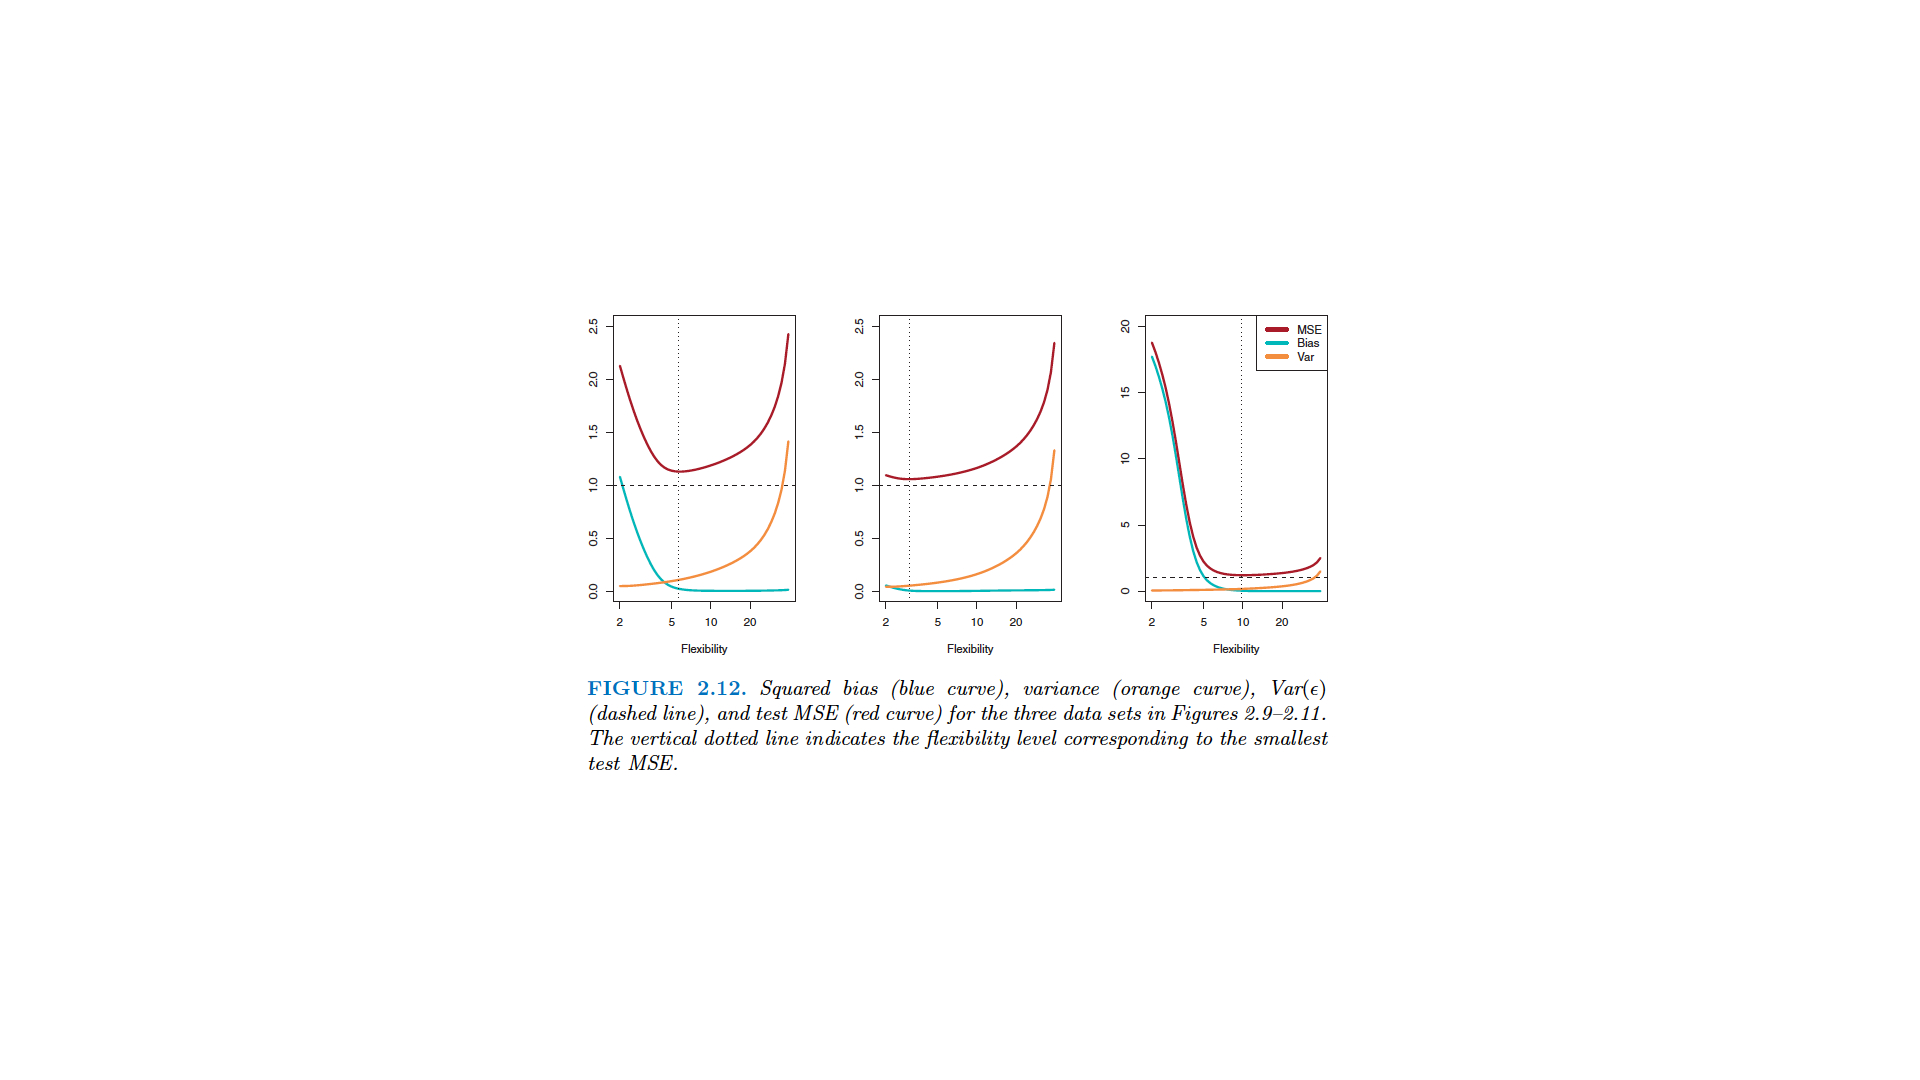
\includegraphics[scale=1.5,width=\linewidth,height=\textheight,keepaspectratio]{Untitled.jpg}
			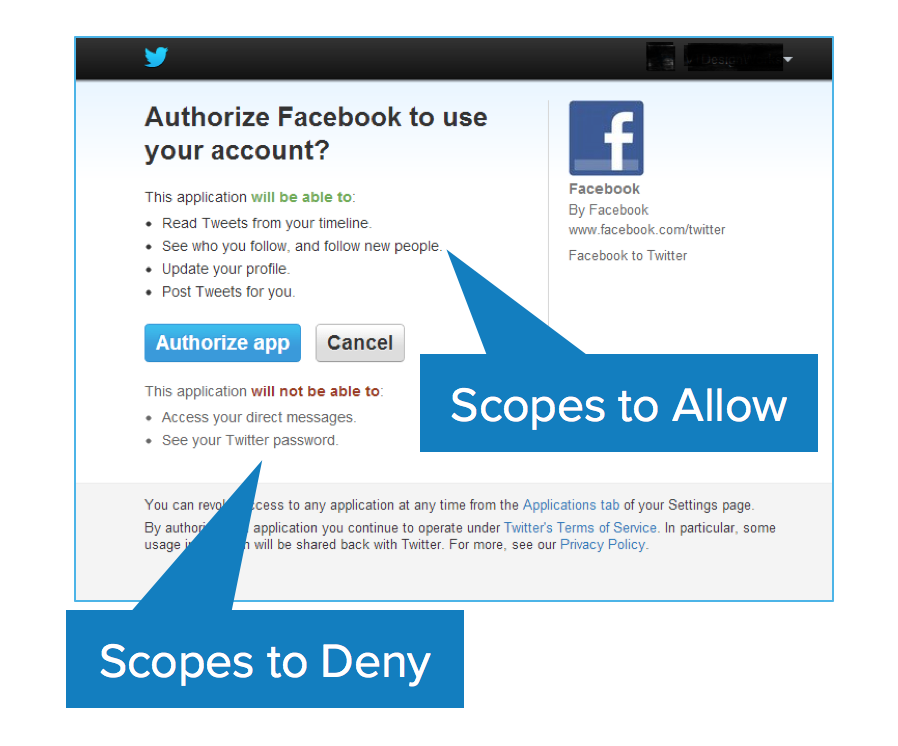
\includegraphics[scale=2.5,height=0.35\paperwidth,keepaspectratio]{oauth-scopes.png}
		\end{figure}
	\end{frame}

	\begin{frame}
		\frametitle{OAuth Actors}
		\begin{itemize}
			\setlength{\itemsep}{20pt}
			\item \textbf{Resource Owner}: owns the data in the resource server. For example, a Gmail user is the Resource Owner of ones account.
			\item \textbf{Resource Server}: The service which stores resouce owner's data. E.g., Gmail.
			\item \textbf{Client}: An application that wants to access your data. E.g., Yelp that wants to fetch your contacts list.
			\item \textbf{Authorization Server}: The main engine of OAuth. Authorization Server is typically administered by a relative of \textbf{Resource Server}
		\end{itemize}
	\end{frame}

	\begin{frame}
		\frametitle{}
		\begin{figure}[hbt!]
			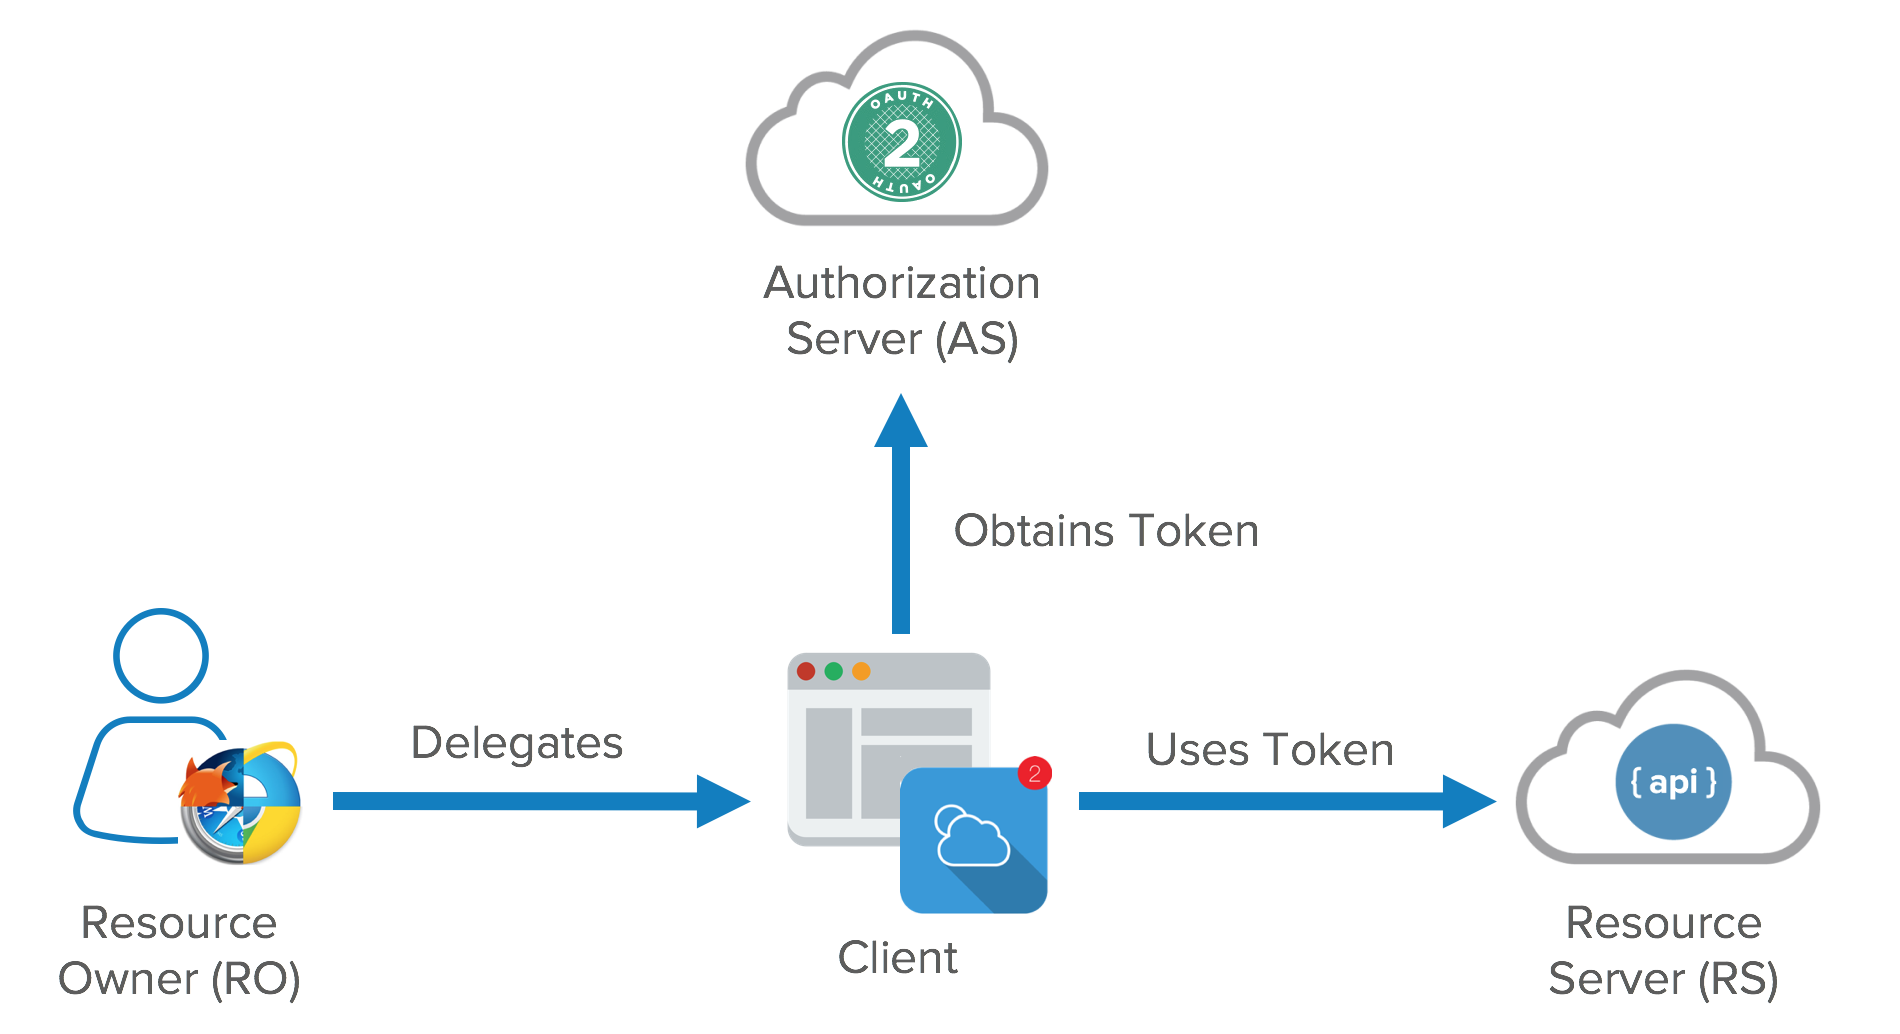
\includegraphics[scale=2.5,height=0.5\paperwidth,keepaspectratio]{oauth-actors.png}
		\end{figure}
			
	\end{frame}

\end{document}